\PassOptionsToPackage{hyphens}{url}
\documentclass{misisarticle}

\usepackage{amsmath, amssymb}
\usepackage{graphicx}
\usepackage{booktabs, array}

\DeclareMathSizes{10}{10}{7}{7}
\DeclareMathSizes{9}{9}{7}{7}
\DeclareMathSizes{8}{8}{7}{7}

\graphicspath{{images/}{./}}

\makeatletter
\@ifundefined{captionsrussian}{%
  \AtBeginDocument{\renewcommand{\refname}{ЛИТЕРАТУРА}}%
}{%
  \addto\captionsrussian{\renewcommand{\refname}{ЛИТЕРАТУРА}}%
}
\makeatother

\grnti{28.23.15}
\asjc{1710, 1712}
\oecd{1.02}

\title{Выявление скрытой предвзятости в моделях кредитного скоринга на основе анализа вклада признаков методами SHAP и LIME}

\misisauthor{Т.~С.~Мухтаров}{кафедра инженерной кибернетики НИТУ «МИСИС»}{Москва, Россия}{m2307203@edu.misis.ru}
\misisauthor{С.~С.~Мишуров}{кафедра инженерной кибернетики НИТУ «МИСИС»}{Москва, Россия}{mishurov.s@misis.ru}

\setabstract{Работа посвящена задаче аудита скрытой (косвенной) предвзятости в моделях кредитного скоринга на основе градиентного бустинга: ситуации, когда защищаемый атрибут (пол или возраст) исключён из входных признаков, но воспроизводится моделью через коррелирующие признаки-прокси. Систематизированы девять методических ограничений применения пост-хок методов объяснимого искусственного интеллекта SHAP и LIME в задачах аудита. Предложена трёхуровневая процедура, разделяющая измерение межгруппового разрыва при фиксированных допустимых факторах риска, отбор кандидатов в прокси по взаимной информации с пермутационным порогом и перекрёстную верификацию знаковых распределений вкладов SHAP и LIME. Работоспособность методики проверена в контролируемом вычислительном эксперименте на датасете UCI Statlog German Credit (4 сценария по 5 прогонов XGBoost). Показано, что уровень измерения не даёт ложных тревог в контрольном сценарии, а модельные детекторы отсекают 100\% синтетических приманок. Строгая гипотеза о превосходстве пересечения SHAP и LIME над каждым методом по отдельности не подтвердилась из-за эффекта потолка точности и наследования пропусков более консервативного объяснителя, что определяет практическую роль пересечения как фильтра точности при сохранении симметрической разности для ручной проверки.}

\setkeywords{кредитный скоринг; скрытая предвзятость; признаки-прокси; аудит моделей; объяснимый искусственный интеллект; SHAP; LIME; градиентный бустинг}

\begin{document}
\maketitle

\section{Введение}

Современные системы кредитного скоринга широко применяют нелинейные ансамблевые алгоритмы, прежде всего градиентный бустинг над решающими деревьями (GBDT), обеспечивающие высокую точность прогнозирования вероятности дефолта. Для соблюдения антидискриминационных требований на практике часто используют стратегию «справедливости через неосведомлённость» (fairness through unawareness), исключая из входных данных защищаемые социально-демографические атрибуты, такие как пол и возраст. Однако подобное исключение не устраняет межгрупповой разрыв в долях одобрений: косвенные признаки (регион проживания, отрасль занятости, канал подачи заявки) несут статистическую информацию о защищаемом атрибуте, и бустинг восстанавливает её при минимизации ошибки на исторических данных.

Регуляторная практика предъявляет к аудиту скоринговых систем два требования одновременно: оценить расхождение решений на сопоставимых заявках и выявить признаки, формирующие это расхождение. В США данная проблематика закреплена в законе ECOA и доктрине неодинакового воздействия (disparate impact)~\cite{barocas2016}, в Европейском союзе — в статье~22 GDPR и регламенте AI Act, относящем оценку кредитоспособности к системам высокого риска.

Вопросы измерения справедливости и компромисса между справедливостью и доходностью в кредитном скоринге подробно исследованы в работах~\cite{kozodoi2022, chen2024}, а задачи интерпретируемого контроля моделей оценки финансовых и операционных рисков — в~\cite{mishurov2023}. Для анализа поведения сложных моделей применяются методы объяснимого искусственного интеллекта (XAI): SHAP на основе значений Шепли~\cite{lundberg2017}, алгоритм TreeSHAP для древовидных ансамблей~\cite{lundberg2020} и локальная линейная аппроксимация LIME~\cite{ribeiro2016}. Прикладные аспекты их использования в задачах классификации и оценивания рисков рассмотрены в~\cite{demin2026, abramov2026}. Вместе с тем в~\cite{slack2020} продемонстрирована уязвимость пост-хок методов на основе возмущений (LIME и KernelSHAP) к преднамеренному искажению объяснений, что делает опору на единственный объяснитель рискованной.

Цель данной работы — разработка и экспериментальная валидация трёхуровневой методики аудита скрытой предвзятости скоринговых моделей, объединяющей условную метрику межгруппового разрыва, пермутационный отбор прокси-признаков и перекрёстную проверку знаковых вкладов SHAP и LIME, а также систематизация методических ловушек XAI-аудита. Исходный код эксперимента, таблицы прогонов и материалы исследования размещены в открытом репозитории:\\
\url{https://github.com/m2307203-creator/credit-scoring-bias-article}.

\section{Механизм скрытой предвзятости и уровни аудита}

\subsection{Формальная постановка и механизм утечки}

Пусть кредитная заявка описывается вектором признаков $X = (X_1, \dots, X_n)$, целевая переменная $Y \in \{0, 1\}$ отражает факт дефолта ($Y = 1$), обученная модель $f$ оценивает вероятность дефолта $P(Y = 1 \mid X)$, а бинарное решение об одобрении задаётся пороговым правилом:
\begin{equation}
D = \mathbf{1}[f(X) < \tau],
\label{eq:decision}
\end{equation}
где $\tau \in (0, 1)$ — установленный порог отсечения. Защищаемый атрибут $A \in \{0, 1\}$ (например, пол или возрастная группа) не входит в пространство признаков модели ($A \notin X$).

Признак $X_i$ выступает статистическим прокси для $A$, если его взаимная информация с защищаемым атрибутом превышает порог существенности: $I(X_i; A) > \varepsilon$. Прокси возникают из статистической структуры социально-экономических данных: территориальные признаки связаны с жилищной сегрегацией, отрасль занятости — с полом, канал подачи заявки и тип устройства — с возрастом и уровнем дохода.

Дополнительно ситуацию осложняют два фактора. Первый — проблема выводов по отклонённым заявкам (reject inference): фактический исход $Y$ наблюдается только для выданных кредитов, вследствие чего историческая избирательность одобрений уже зафиксирована в обучающих метках. Второй фактор заключается в том, что скрытая предвзятость формируется не изолированно в весах классификатора, а в связке «данные + модель + порог $\tau$»: одна и та же модель при изменении $\tau$ демонстрирует различный межгрупповой разрыв. Механизм возникновения скрытой предвзятости показан на рис.~\ref{fig:mechanism}.

\begin{figure*}[t]
\centering
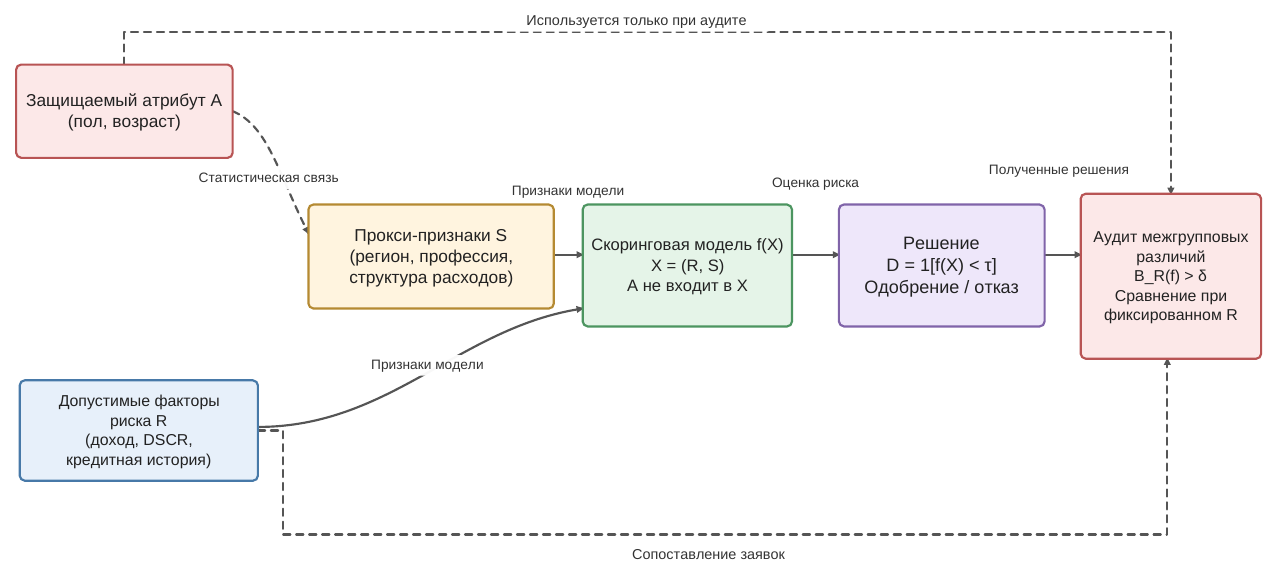
\includegraphics[width=0.92\textwidth]{fig_mechanism.png}
\caption{Механизм возникновения скрытой предвзятости. Защищаемый атрибут $A$ исключён из $X$, но статистически связан с прокси-признаками $S$; модель на $X = (R, S)$ формирует решение $D$; аудит сравнивает группы при фиксированных допустимых факторах риска $R$.}
\label{fig:mechanism}
\end{figure*}

Само наличие прокси не доказывает дискриминацию, но создаёт канал, через который информация об $A$ способна влиять на решения модели и который подлежит раздельной проверке.

\subsection{Разделение уровней аудита}

Распространённой методологической ошибкой является объединение различных вопросов аудита в одно утверждение вида «признак имеет высокий SHAP и коррелирует с полом, следовательно, модель предвзята». Корректная процедура строго разделяет три уровня анализа (табл.~\ref{tab:levels} и рис.~\ref{fig:pipeline}).

\begin{table*}[t]
\centering
\caption{Три уровня аудита скрытой предвзятости и границы выводов каждого уровня}
\label{tab:levels}
\footnotesize
\begin{tabular}{@{} >{\raggedright\arraybackslash}p{0.18\textwidth} >{\raggedright\arraybackslash}p{0.31\textwidth} >{\raggedright\arraybackslash}p{0.18\textwidth} >{\raggedright\arraybackslash}p{0.25\textwidth} @{}}
\toprule
Уровень & Решаемый вопрос & Инструмент & Чего уровень не доказывает \\
\midrule
1. Измерение & Есть ли значимый разрыв в одобрениях на сопоставимых заявках? & $B_R(f)$, DP / EOp / EO & Через какие признаки возник разрыв \\
2. Прокси-анализ (данные) & Какие признаки несут информацию об $A$? & Взаимная информация $I(X_i; A)$ & Использует ли их сама модель \\
3. Вклад (модель) & На какие признаки модель реально опирается? & SHAP, LIME & Есть ли дискриминация и причинна ли она \\
\bottomrule
\end{tabular}
\end{table*}

\begin{figure*}[t]
\centering
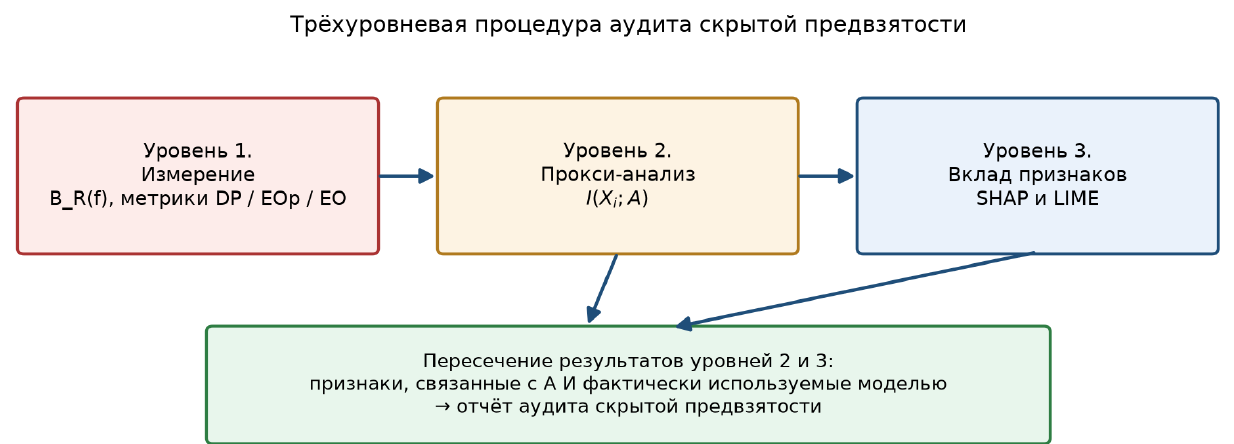
\includegraphics[width=0.88\textwidth]{fig_pipeline.png}
\caption{Трёхуровневая процедура аудита скрытой предвзятости. В итоговый отчёт попадает пересечение результатов уровней 2 и 3 — признаки, одновременно статистически связанные с $A$ и фактически используемые моделью.}
\label{fig:pipeline}
\end{figure*}

Методы SHAP и LIME отвечают исключительно на вопрос третьего уровня, описывая механику обученной модели. Они не заменяют групповые метрики справедливости и не устанавливают причинную дискриминацию.

\subsection{Определение предвзятости и несовместимость метрик}

Разделим вектор признаков на $X = (R, S)$, где $R$ — экономически обоснованные допустимые факторы риска (доход, долговая нагрузка, кредитная история), а $S$ — остальные признаки. Операциональное определение скрытой предвзятости основано на условном статистическом паритете:
\begin{equation}
\begin{aligned}
B_R(f) = \mathbb{E}_{r \sim Q}\bigl|\,&P(D = 1 \mid A = 1, R = r) \\
&- P(D = 1 \mid A = 0, R = r)\bigr| > \delta,
\end{aligned}
\label{eq:bias}
\end{equation}
где $Q$ — распределение допустимых факторов, а $\delta > 0$ — пороговый уровень диспаритета. Условие~\eqref{eq:bias} означает, что среди заявок с одинаковыми допустимыми факторами риска вероятности одобрения между группами расходятся в среднем сильнее, чем на $\delta$. Такой подход переводит возражение кредитной организации «различия объясняются уровнем риска» в проверяемую плоскость при условии, что выбранный набор факторов $R$ действительно полно описывает кредитный риск.

Применение определения~\eqref{eq:bias} требует соблюдения четырёх ограничений: нормативные параметры $(R, Q, \tau, \delta)$ фиксируются до запуска аудита; превышение $\delta$ трактуется как диагностический сигнал, а не юридическое заключение; при высокой размерности $R$ стратификация сталкивается с нехваткой сопоставимых заявок в обеих группах; защищаемый атрибут $A$ доступен только аудитору и не подаётся на вход модели.

Выражение~\eqref{eq:bias} обобщает классические критерии справедливости (табл.~\ref{tab:fairness}): при $R = \emptyset$ оно сводится к демографическому паритету (DP), а при $R = Y$ — к уравненным шансам (EO), однако истинный исход $Y$ известен лишь ретроспективно. Если базовые доли дефолта $P(Y = 1 \mid A = a)$ в группах различаются, критерии DP и EO математически несовместимы~\cite{hardt2016, verma2018}, за исключением вырожденных моделей, не зависящих от исхода. Для кредитного скоринга в работе~\cite{kozodoi2022} рекомендуется использовать критерий разделения (separation, EO).

\begin{table}[t]
\centering
\caption{Критерии справедливости и их основные ограничения}
\label{tab:fairness}
\footnotesize
\begin{tabular}{@{} >{\raggedright\arraybackslash}p{0.17\columnwidth} >{\raggedright\arraybackslash}p{0.34\columnwidth} >{\raggedright\arraybackslash}p{0.37\columnwidth} @{}}
\toprule
Критерий & Требование & Ограничение \\
\midrule
DP & Равные доли одобрений & Игнорирует разницу рисков \\
EOp & Равные одобрения среди $Y = 0$ & Не контролирует ошибки по дефолтникам \\
EO & Равенство ошибок при $Y \in \{0, 1\}$ & Требует знания $Y$ ретроспективно \\
$B_R(f)$ & Равенство при фиксированном $R$ & Выбор $R, Q$ и проклятие размерности \\
\bottomrule
\end{tabular}
\end{table}

\section{Методические ограничения и ловушки XAI-аудита}

Ниже систематизированы девять типовых проблем, приводящих к ошибочным выводам при использовании SHAP и LIME в аудите скоринговых моделей.

\subsection{Выбор постановки и шкалы выхода (ловушки 1 и 2)}

Метод SHAP опирается на значения Шепли — средний маржинальный вклад признака по всем коалициям~\cite{lundberg2017}. В интервенциональной постановке отсутствующие признаки подставляются из фоновой выборки $z^{(b)}$:
\begin{equation}
v_x(S) = \frac{1}{m}\sum_{b=1}^{m} f\bigl(x_S,\, z_{-S}^{(b)}\bigr).
\label{eq:interventional}
\end{equation}
В интервенциональном режиме признак, не используемый моделью, гарантированно получает нулевой вклад, тогда как в условной постановке коррелированный неиспользуемый признак может получить ненулевую атрибуцию. Для задач аудита предпочтителен интервенциональный режим, проверяющий фактическое использование признака моделью.

\emph{Ловушка 1 (фоновая выборка).} Значения SHAP зависят от состава фоновой выборки. Размер фона и генератор случайных чисел (\texttt{seed}) необходимо фиксировать в протоколе аудита для воспроизводимости.

\emph{Ловушка 2 (шкала выхода).} Свойство полноты разложения выполняется как для вероятностной шкалы, так и для шкалы лог-шансов (логита):
\begin{equation}
\sum_{i} \varphi_i(f, x) = f(x) - \mathbb{E}[f(X)].
\label{eq:efficiency}
\end{equation}
Величины вкладов на разных шкалах существенно различаются, поэтому объясняемый выход фиксируется заранее (в данной работе используется шкала логита, \texttt{model\_output="raw"}).

\subsection{Корреляции и кодирование признаков (ловушки 3 и 4)}

\emph{Ловушка 3 (коррелированные прокси).} Прокси-признаки коррелируют с $A$ и часто между собой. SHAP распределяет вклад между коллинеарными столбцами: при удалении одного прокси его вес перераспределяется на соседние, а выход модели почти не меняется. Анализ признаков строго по одному не выявляет такую взаимозаменяемость.

\emph{Ловушка 4 (фрагментация one-hot-кодирования).} Категориальная переменная после one-hot-кодирования распадается на множество фиктивных столбцов, каждый из которых выглядит малозначимым. На практике вклады фиктивных столбцов суммируются обратно по исходному признаку: это общепринятый приём, сохраняющий свойство полноты~\eqref{eq:efficiency} для всей модели, хотя математически сумма значений Шепли по отдельным столбцам не тождественна значению Шепли для исходной категориальной переменной.

\subsection{Ограничения LIME на табличных данных (ловушка 5)}

\emph{Ловушка 5 (возмущения вне носителя данных).} На табличных данных LIME~\cite{ribeiro2016} сэмплирует признаки независимо, порождая нереалистичные комбинации (например, высокий доход при нулевом стаже или несовместимые категории). Локальный суррогат частично обучается вне носителя реального распределения. Кроме того, коэффициенты LIME не обладают свойством полноты, поэтому их прямое сравнение со значениями SHAP по модулю некорректно — допустима лишь перекрёстная проверка по составу и рангам значимых признаков.

\subsection{Границы интерпретации и манипулируемость (ловушки 6--9)}

\emph{Ловушка 6 (нестабильность и манипулируемость).} Оценки LIME зависят от \texttt{seed} генерации возмущений. Кроме того, в~\cite{slack2020} показаны состязательные атаки на пертурбационные объяснители (LIME и KernelSHAP): модель-обёртка распознаёт синтетические возмущения и маскирует смещение на них, оставаясь предвзятой на реальных заявках. Хотя атаки в~\cite{slack2020} не применялись к TreeSHAP, полагаться в аудите на единственный метод рискованно.

\emph{Ловушка 7 (отсутствие эталона важности).} В работе~\cite{kumar2020} показано, что значения Шепли могут расходиться с интуитивным понятием важности признака, поэтому их следует трактовать как диагностический индикатор, а не окончательное доказательство.

\emph{Ловушка 8 (отсутствие причинного статуса).} Атрибуции SHAP и LIME отражают статистические связи в данных и механику модели; для юридических выводов они применимы лишь как источник проверяемых гипотез.

\emph{Ловушка 9 (потеря знака при глобальном усреднении).} Стандартная метрика $\mathrm{mean}(|\mathrm{SHAP}|)$ скрывает ситуацию, когда прокси повышает вероятность одобрения одной группе и понижает другой. В аудите необходимо сравнивать знаковые распределения вкладов отдельно по группам:
\begin{equation}
\Phi_j^{(a)} = \{\varphi_j(x_k) \mid a_k = a\}, \quad a \in \{0, 1\}.
\label{eq:signed_groups}
\end{equation}

\section{Архитектура пайплайна $\text{SHAP} \cap \text{LIME}$}

На уровне 1 вычисляется условный диспаритет $B_R(f)$ путём стратификации по допустимым факторам $R$ (тертилям суммы и срока кредита) и сравнивается с шумовым порогом $\delta$ (95-й перцентиль при 200 случайных перестановках $A$). На уровне 2 отбираются кандидаты в прокси по взаимной информации $I(X_i; A) > \varepsilon$, где $\varepsilon$ задаётся как 95-й перцентиль максимума MI по 50 перестановкам $A$.

На уровне 3 основным детектором выступает интервенциональный TreeSHAP~\cite{lundberg2020}, а независимой проверкой — LIME. Итоговый список формируется их пересечением, тогда как признаки из симметрической разности передаются риск-аналитику на ручную проверку. Контрфактические объяснения~\cite{wachter2018} целесообразно оставлять для разбора индивидуальных отказов.

Расчёт интервенционального TreeSHAP на шкале логита по отложенной матрице \texttt{M\_test} (400 строк) с фиксированным фоном \texttt{background} (100 строк обучающей выборки) и агрегацией one-hot-столбцов:

\par\vspace{3pt}
\noindent\begin{minipage}{\columnwidth}
\noindent\rule{\linewidth}{0.4pt}
\begingroup
\scriptsize
\begin{verbatim}
explainer = shap.TreeExplainer(
    model,
    data=background,
    feature_perturbation="interventional",
    model_output="raw",
)
vals = explainer.shap_values(M_test)
phi = aggregate(vals, enc.groups, enc.features)
\end{verbatim}
\endgroup
\vspace{-4pt}
\noindent\rule{\linewidth}{0.4pt}
\end{minipage}
\par\vspace{4pt}

Сравнение знаковых распределений вкладов~\eqref{eq:signed_groups} между группами выполняется двумя непараметрическими тестами — Колмогорова--Смирнова и Манна--Уитни — с поправкой Бенджамини--Хохберга ($\alpha = 0{,}05$) и порогом размера эффекта $0{,}10$, отсекающим практически незначимые смещения:

\par\vspace{3pt}
\noindent\begin{minipage}{\columnwidth}
\noindent\rule{\linewidth}{0.4pt}
\begingroup
\scriptsize
\begin{verbatim}
def group_flags(attr, a):
    g0, g1 = attr[a == 0], attr[a == 1]
    n_feat = attr.shape[1]
    p_ks = np.ones(n_feat)
    p_mw = np.ones(n_feat)
    effect = np.zeros(n_feat)
    for j in range(n_feat):
        if np.ptp(attr[:, j]) == 0:
            continue
        p_ks[j] = ks_2samp(
            g0[:, j], g1[:, j]
        ).pvalue
        res = mannwhitneyu(g0[:, j], g1[:, j])
        p_mw[j] = res.pvalue
        effect[j] = abs(
            res.statistic
            / (len(g0) * len(g1)) - 0.5
        )
    return (
        (bh_adjust(p_ks) < 0.05)
        & (bh_adjust(p_mw) < 0.05)
        & (effect >= 0.10)
    )
\end{verbatim}
\endgroup
\vspace{-4pt}
\noindent\rule{\linewidth}{0.4pt}
\end{minipage}
\par\vspace{4pt}

Перекрёстная верификация (LIME рассчитывается на стратифицированной подвыборке \texttt{a\_lime} из 200 строк — по 100 на группу):

\par\vspace{3pt}
\noindent\begin{minipage}{\columnwidth}
\noindent\rule{\linewidth}{0.4pt}
\begingroup
\scriptsize
\begin{verbatim}
candidates = mi > eps
p_shap = candidates & group_flags(
    phi_shap, a_test
)
p_lime = candidates & group_flags(
    phi_lime, a_lime
)
p_cross = p_shap & p_lime
to_review = p_shap ^ p_lime
\end{verbatim}
\endgroup
\vspace{-4pt}
\noindent\rule{\linewidth}{0.4pt}
\end{minipage}
\par\vspace{4pt}

\section{Постановка вычислительного эксперимента}

Проверяемая строгая гипотеза $H_1$ формулируется следующим образом: пересечение $\text{SHAP} \cap \text{LIME}$ обеспечивает более высокую точность ($\text{precision}$) выявления фактически используемых моделью прокси по сравнению с корреляционным фильтром MI и каждым объяснителем по отдельности при сохранении полноты ($\text{recall}$, TPR) не ниже $0{,}9$ от максимальной среди сравниваемых методов:
\begin{equation}
\begin{aligned}
\text{precision} &= \frac{|\widehat{P} \cap P^*|}{|\widehat{P}|}, \quad
\text{recall} = \frac{|\widehat{P} \cap P^*|}{|P^*|}, \\
\text{FPR} &= \frac{|\widehat{P} \setminus P^*|}{d - |P^*|},
\end{aligned}
\label{eq:metrics}
\end{equation}
где $\widehat{P}$ — множество выявленных признаков, $P^*$ — эталонное множество прокси, реально используемых моделью. Независимость ошибок SHAP и LIME заранее не предполагается.

Поскольку на реальных данных состав $P^*$ неизвестен, построена серия контролируемых сценариев на датасете UCI Statlog German Credit~\cite{germancredit} (1000 записей, 20 исходных признаков). В общей постановке защищаемым атрибутом может выступать как пол, так и возраст; в данном эксперименте зафиксировано $A = \text{пол}$ (извлечённый из \texttt{personal\_status} и исключённый из входов модели), что позволяет проследить появление возраста (\texttt{age}) в роли естественного прокси. Параметры четырёх сценариев сведены в табл.~\ref{tab:scenarios}.

\begin{table}[t]
\centering
\caption{Контролируемые сценарии эксперимента на UCI German Credit}
\label{tab:scenarios}
\footnotesize
\begin{tabular}{@{} >{\raggedright\arraybackslash}p{0.21\columnwidth} >{\raggedright\arraybackslash}p{0.44\columnwidth} >{\raggedright\arraybackslash}p{0.25\columnwidth} @{}}
\toprule
Сценарий & Внедрённые признаки & Цель проверки \\
\midrule
Контроль & 0 внедрённых прокси, 2 шума (естественные связи сохранены) & Проверка FPR \\
Слабая связь & 2 используемых ($\rho = 0{,}30$), 2 приманки, 2 шума & Порог чувствительности \\
Умеренная связь & 3 используемых ($\rho = 0{,}55$), 2 приманки, 2 шума & Баланс TPR и FPR \\
Сильная связь & 3 используемых ($\rho = 0{,}85$), 2 приманки, 2 шума & Верхняя оценка TPR \\
\bottomrule
\end{tabular}
\end{table}

Целевые метки дефолта синтезированы из базовой логит-модели German Credit с добавлением вклада используемых прокси (\texttt{proxy\_used}). В каждый сценарий со связью добавлены две синтетические «приманки» (\texttt{proxy\_decoy}, корреляция с $A$ около $0{,}70$). Чтобы гарантировать их статистическую связь с $A$ при полном отсутствии использования моделью, столбцы приманок обнуляются на этапе обучения и возвращаются в исходном виде при аудите:

\par\vspace{3pt}
\noindent\begin{minipage}{\columnwidth}
\noindent\rule{\linewidth}{0.4pt}
\begingroup
\scriptsize
\begin{verbatim}
M_tr_fit = mask_decoys(M_tr, enc, decoys)
model = fit_model(
    M_tr_fit, y[idx_tr], seed, kind
)
verified, max_decoy_gain = verified_truth(
    model, enc, used, decoys
)
\end{verbatim}
\endgroup
\vspace{-4pt}
\noindent\rule{\linewidth}{0.4pt}
\end{minipage}
\par\vspace{4pt}

Эталон $P^*$ подтверждается по фактической доле суммарного прироста в разбиениях обученного XGBoost (\texttt{total\_gain} $\ge 0{,}01$), что, в отличие от одиночной перестановочной важности, устойчиво к мультиколлинеарности прокси. Всего выполнено 20 прогонов (4 сценария $\times$ 5 значений \texttt{seed} 2026--2030) при пороге одобрения $\tau = 0{,}30$; TreeSHAP рассчитывался по 400 строкам тестовой выборки, LIME (600 возмущений на объект) — по 200 строкам.

\section{Результаты экспериментов и обсуждение}

\subsection{Уровень 1: измерение межгрупповых различий}

Результаты работы первого уровня аудита представлены в табл.~\ref{tab:level1} и на рис.~\ref{fig:level1}. Порог $\delta$ отражает 95-й перцентиль $B_R(f)$ при перемешанном $A$. По отдельным прогонам ROC-AUC моделей XGBoost находился в диапазоне $0{,}76\text{--}0{,}84$.

\begin{table*}[t]
\centering
\caption{Уровень 1: межгрупповой разрыв одобрений и частота сигнала по сценариям (среднее $\pm$ $\sigma$ по 5 прогонам)}
\label{tab:level1}
\footnotesize
\begin{tabular}{@{} l c c c c c c c @{}}
\toprule
Сценарий & ROC-AUC & $B_R(f)$ & Порог $\delta$ & Разность DP & EO ($Y = 0$) & EO ($Y = 1$) & Сигнал ($B_R > \delta$) \\
\midrule
Контроль & $0{,}787 \pm 0{,}031$ & $0{,}115 \pm 0{,}044$ & $0{,}166 \pm 0{,}006$ & $0{,}050 \pm 0{,}063$ & $0{,}054 \pm 0{,}056$ & $0{,}087 \pm 0{,}113$ & 0 из 5 \\
Слабая связь & $0{,}790 \pm 0{,}013$ & $0{,}187 \pm 0{,}060$ & $0{,}164 \pm 0{,}007$ & $0{,}158 \pm 0{,}057$ & $0{,}115 \pm 0{,}079$ & $0{,}094 \pm 0{,}042$ & 4 из 5 \\
Умеренная связь & $0{,}805 \pm 0{,}022$ & $0{,}318 \pm 0{,}031$ & $0{,}168 \pm 0{,}008$ & $0{,}296 \pm 0{,}024$ & $0{,}175 \pm 0{,}026$ & $0{,}216 \pm 0{,}089$ & 5 из 5 \\
Сильная связь & $0{,}809 \pm 0{,}013$ & $0{,}413 \pm 0{,}063$ & $0{,}168 \pm 0{,}007$ & $0{,}395 \pm 0{,}049$ & $0{,}259 \pm 0{,}078$ & $0{,}324 \pm 0{,}112$ & 5 из 5 \\
\bottomrule
\end{tabular}
\end{table*}

\begin{figure*}[t]
\centering
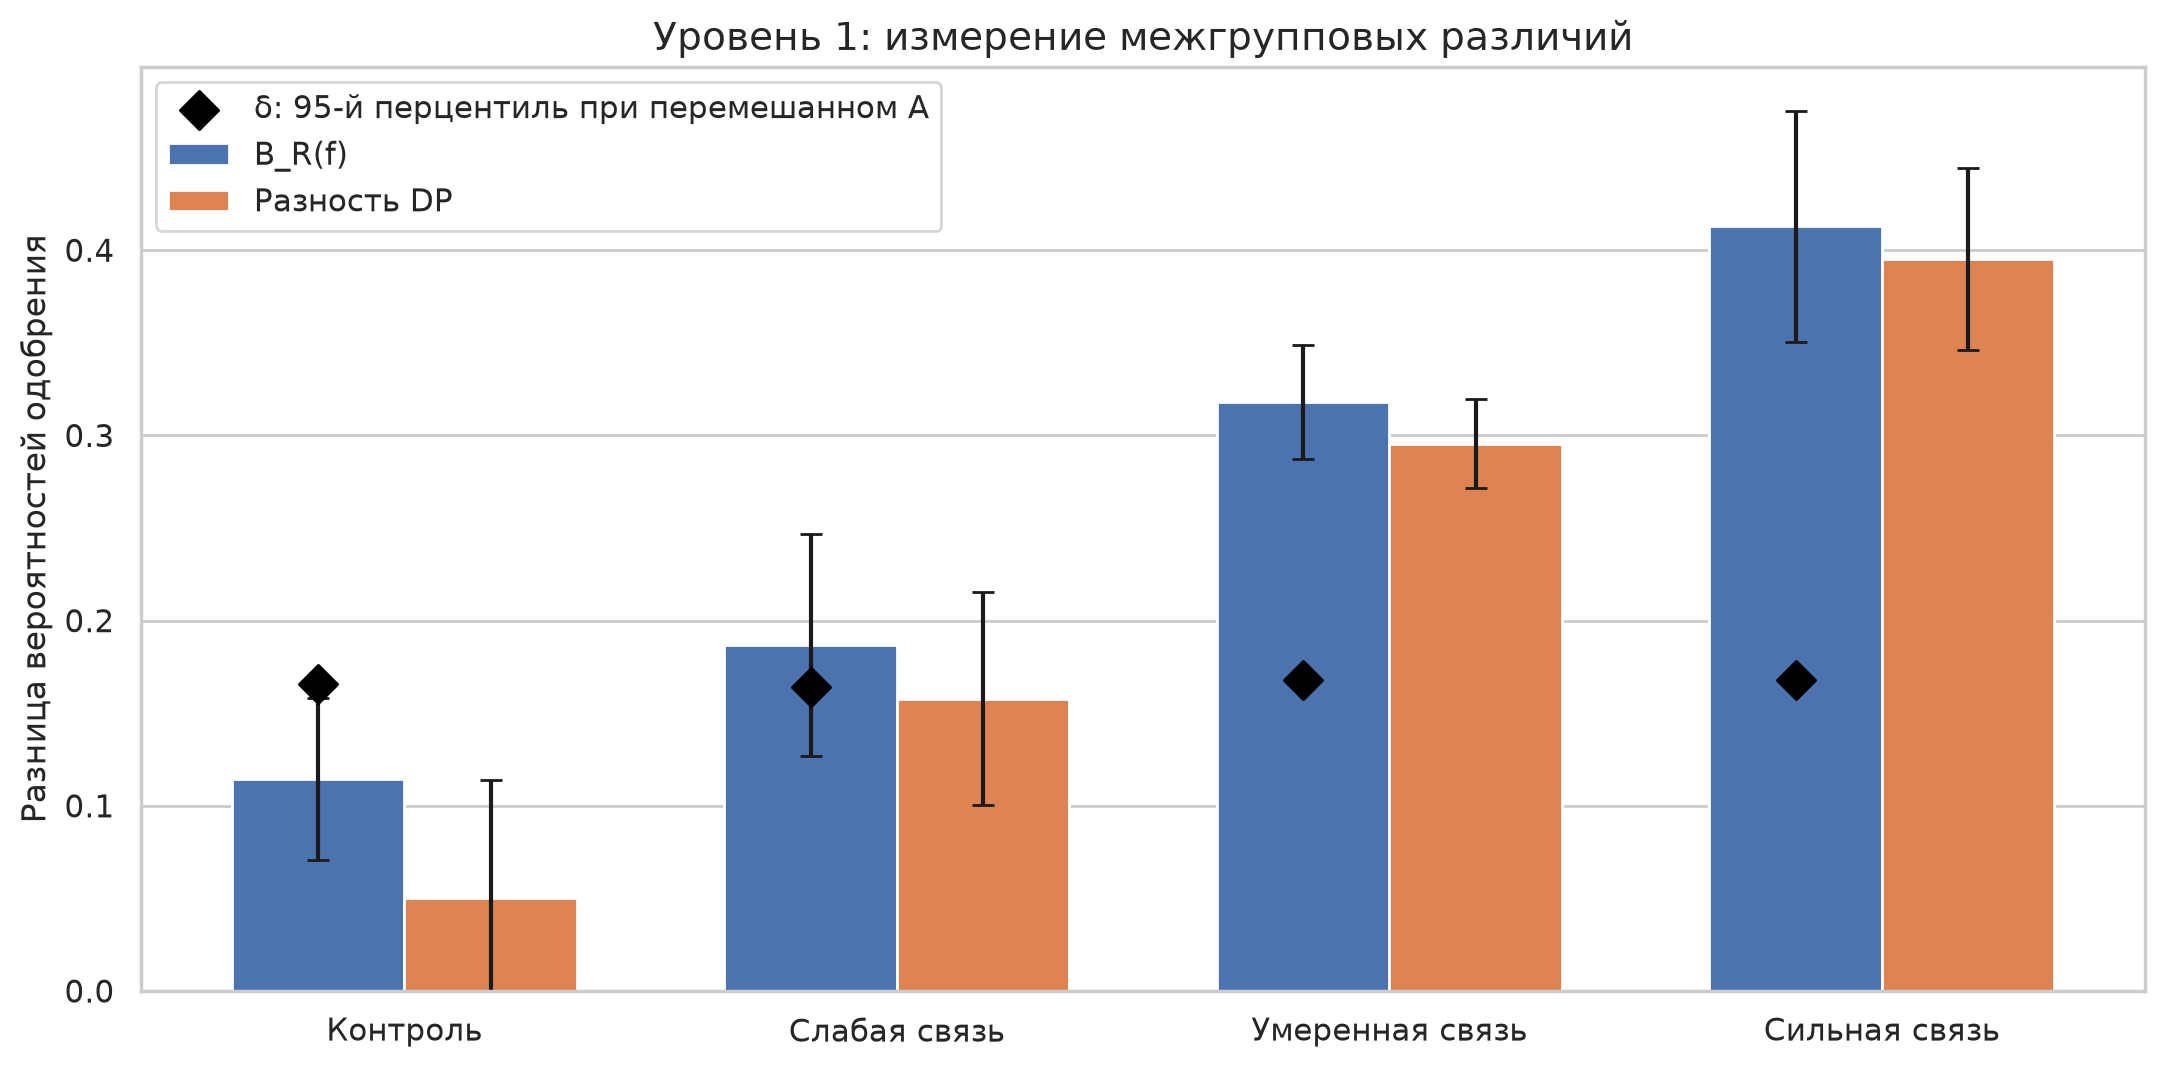
\includegraphics[width=0.90\textwidth]{fig3_level1_measurement.png}
\caption{Уровень 1: средние значения $B_R(f)$ и разности DP ($\pm\sigma$ по 5 прогонам) на фоне шумового порога $\delta$ (чёрные ромбы). В контрольном сценарии оба показателя ниже порога; в умеренной и сильной связи разрыв стабильно превышает шум.}
\label{fig:level1}
\end{figure*}

В контрольном сценарии уровень 1 не дал ни одной ложной тревоги (0 из 5 прогонов: $B_R \approx 0{,}115$ при $\delta \approx 0{,}166$). При умеренной и сильной связи сигнал зафиксирован в 5 из 5 прогонов, а при слабой связи — в 4 из 5.

Выполнена проверка двух вычислительных инвариантов по всем 20 прогонам: максимальное расхождение аддитивности TreeSHAP~\eqref{eq:efficiency} составило $4{,}29 \cdot 10^{-6}$ (уровень точности \texttt{float32}), а максимальная доля \texttt{total\_gain} у приманок \texttt{proxy\_decoy} равна ровно $0{,}0$, что подтверждает их полное неиспользование обученными моделями.

\subsection{Уровни 2 и 3: обнаружение прокси-признаков}

Сводные метрики выявления прокси-признаков приведены в табл.~\ref{tab:detection} и на рис.~\ref{fig:metrics}. В контрольном сценарии множество $P^*$ пусто, поэтому $\text{recall}$ не определён (н/д), а $\text{precision}$ равен нулю во всех $n$ прогонах, где метод выдал хотя бы одно срабатывание.

\begin{table*}[t]
\centering
\caption{Уровни 2 и 3: показатели Precision, Recall (TPR) и FPR по методам и сценариям (среднее $\pm$ $\sigma$ по 5 прогонам)}
\label{tab:detection}
\footnotesize
\begin{tabular}{@{} l l c c c @{}}
\toprule
Сценарий & Метод & Precision & Recall (TPR) & FPR \\
\midrule
Контроль & Корреляция (MI) & $0{,}000 \pm 0{,}000\;(n=4)$ & н/д & $0{,}067 \pm 0{,}054$ \\
Контроль & SHAP & $0{,}000 \pm 0{,}000\;(n=2)$ & н/д & $0{,}019 \pm 0{,}026$ \\
Контроль & LIME & $0{,}000\;(n=1)$ & н/д & $0{,}019 \pm 0{,}043$ \\
Контроль & $\text{SHAP} \cap \text{LIME}$ & $0{,}000\;(n=1)$ & н/д & $0{,}010 \pm 0{,}021$ \\
\midrule
Слабая связь & Корреляция (MI) & $0{,}393 \pm 0{,}068$ & $1{,}000 \pm 0{,}000$ & $0{,}139 \pm 0{,}036$ \\
Слабая связь & SHAP & $0{,}833 \pm 0{,}236$ & $0{,}900 \pm 0{,}224$ & $0{,}017 \pm 0{,}024$ \\
Слабая связь & LIME & $0{,}900 \pm 0{,}224$ & $0{,}800 \pm 0{,}274$ & $0{,}009 \pm 0{,}019$ \\
Слабая связь & $\text{SHAP} \cap \text{LIME}$ & $0{,}900 \pm 0{,}224$ & $0{,}800 \pm 0{,}274$ & $0{,}009 \pm 0{,}019$ \\
\midrule
Умеренная связь & Корреляция (MI) & $0{,}540 \pm 0{,}055$ & $1{,}000 \pm 0{,}000$ & $0{,}113 \pm 0{,}024$ \\
Умеренная связь & SHAP & $1{,}000 \pm 0{,}000$ & $0{,}933 \pm 0{,}149$ & $0{,}000 \pm 0{,}000$ \\
Умеренная связь & LIME & $1{,}000 \pm 0{,}000$ & $1{,}000 \pm 0{,}000$ & $0{,}000 \pm 0{,}000$ \\
Умеренная связь & $\text{SHAP} \cap \text{LIME}$ & $1{,}000 \pm 0{,}000$ & $0{,}933 \pm 0{,}149$ & $0{,}000 \pm 0{,}000$ \\
\midrule
Сильная связь & Корреляция (MI) & $0{,}540 \pm 0{,}055$ & $1{,}000 \pm 0{,}000$ & $0{,}113 \pm 0{,}024$ \\
Сильная связь & SHAP & $0{,}850 \pm 0{,}137$ & $1{,}000 \pm 0{,}000$ & $0{,}026 \pm 0{,}024$ \\
Сильная связь & LIME & $1{,}000 \pm 0{,}000$ & $1{,}000 \pm 0{,}000$ & $0{,}000 \pm 0{,}000$ \\
Сильная связь & $\text{SHAP} \cap \text{LIME}$ & $1{,}000 \pm 0{,}000$ & $1{,}000 \pm 0{,}000$ & $0{,}000 \pm 0{,}000$ \\
\bottomrule
\end{tabular}
\end{table*}

Совпадение показателей корреляционного фильтра MI в умеренной и сильной связи до тысячных объясняется тем, что на одних и тех же \texttt{seed} (2026--2030) взаимная информация отбирает идентичный набор из 5--6 признаков (три \texttt{proxy\_used}, две \texttt{proxy\_decoy} и поочерёдно \texttt{age} или \texttt{num\_dependents}), поскольку при обеих силах связи все внедрённые прокси и приманки уверенно превышают пермутационный порог $\varepsilon$.

\begin{figure*}[t]
\centering
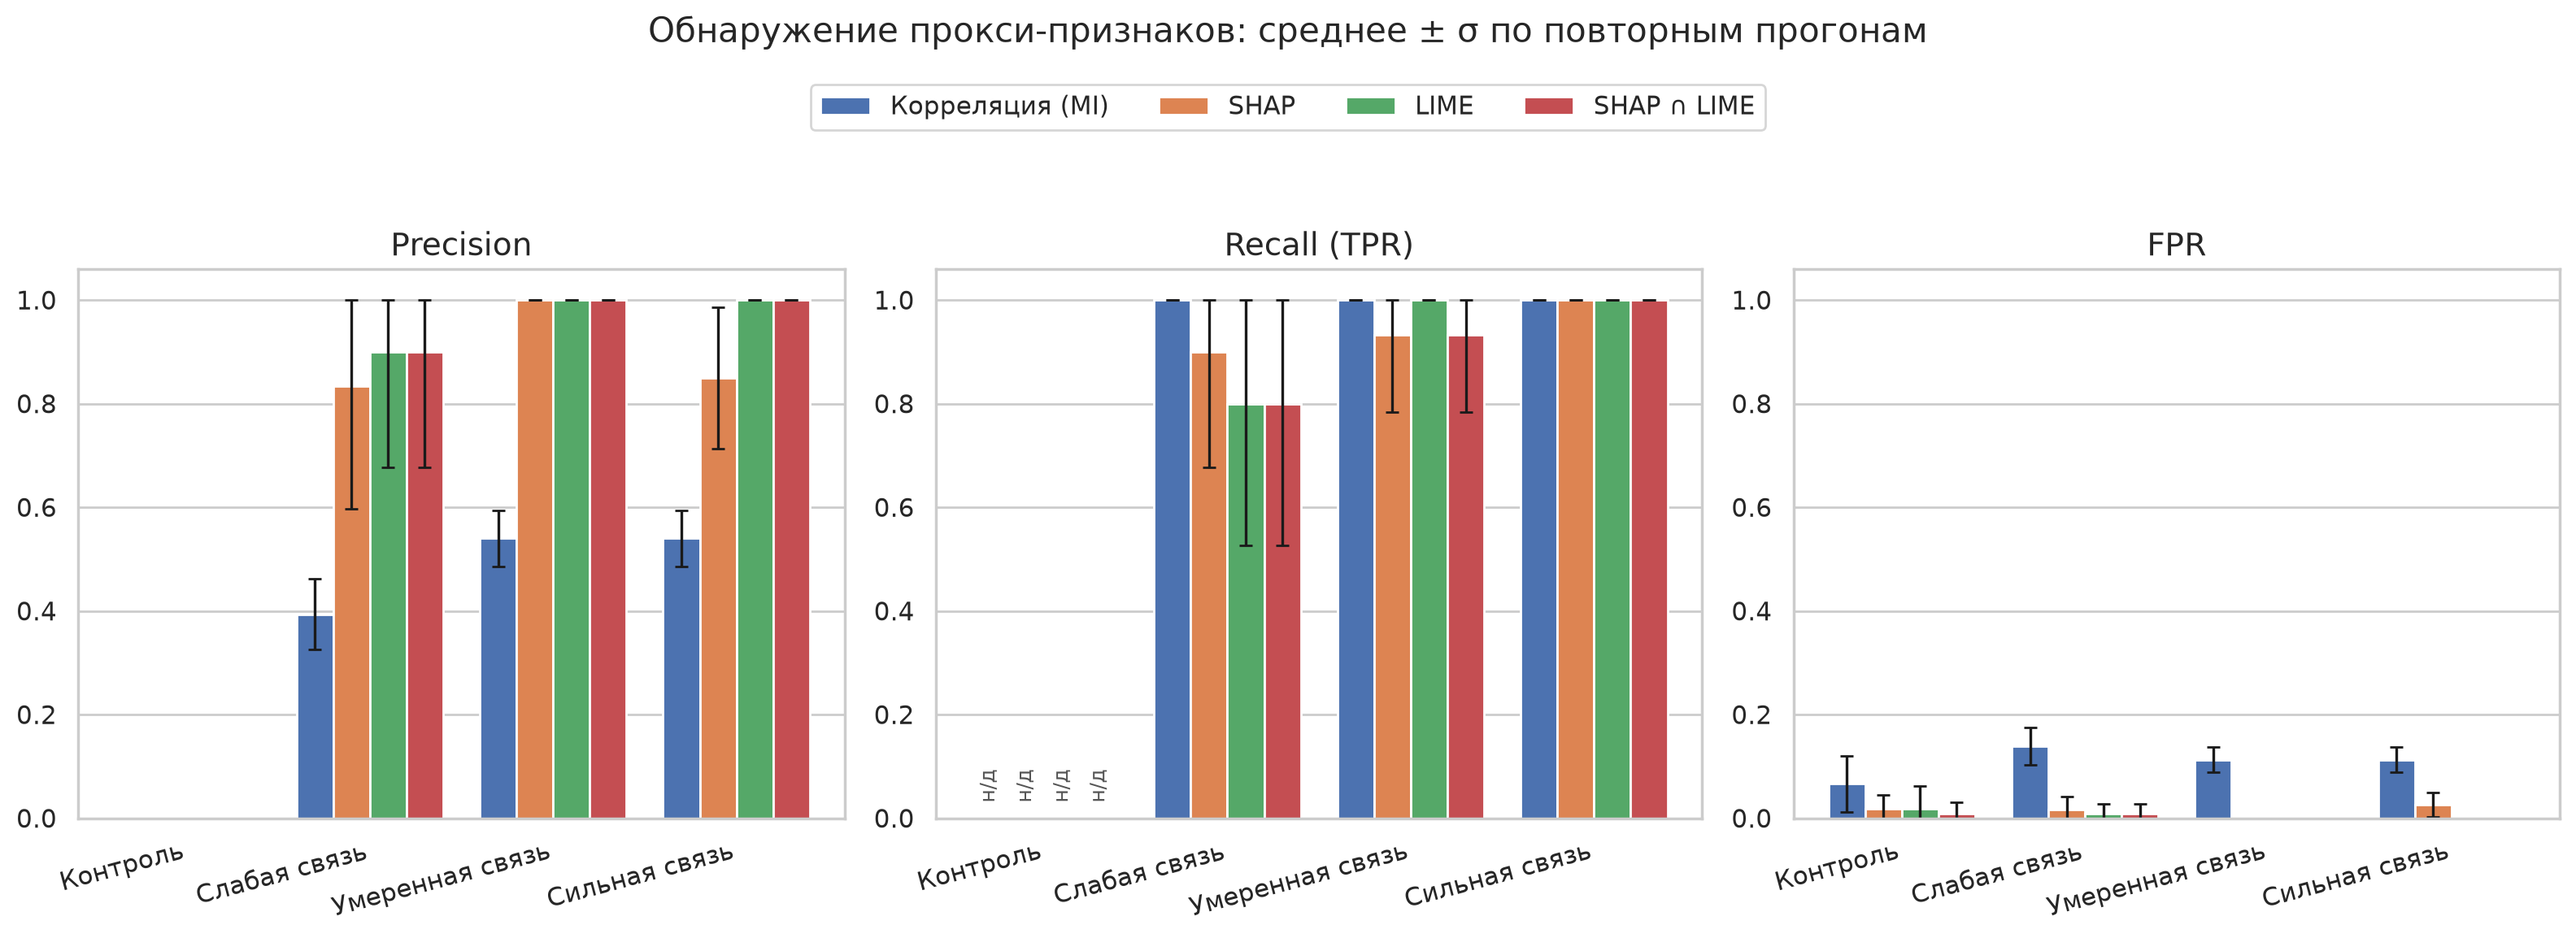
\includegraphics[width=0.95\textwidth]{fig1_precision_recall_fpr.png}
\caption{Precision, Recall (TPR) и FPR по методам и сценариям (среднее $\pm\sigma$). В контрольном сценарии Recall не определён (н/д) из-за пустого эталона $P^*$. Корреляционный фильтр MI удерживает Recall на уровне $1{,}000$, но демонстрирует Precision $0{,}39\text{--}0{,}54$ и FPR $0{,}11\text{--}0{,}14$.}
\label{fig:metrics}
\end{figure*}

\subsection{Анализ гипотезы $H_1$ и естественных прокси}

\emph{Проверка гипотезы $H_1$.} Строгое условие $H_1$ ($\text{precision}(\text{SHAP} \cap \text{LIME}) > \max$ остальных при $\text{recall} \ge 0{,}9 \cdot \max$) не выполнилось ни в одном прогоне (доля $0{,}0$). В умеренной и сильной связи сработал эффект потолка: LIME самостоятельно достиг $\text{precision} = 1{,}000$, и строго превзойти единицу математически невозможно. При ослаблении неравенства до нестрогого ($\ge$) условие выполняется в $0{,}6$ прогонов слабого, $0{,}8$ умеренного и $1{,}0$ сильного сценария.

При этом практический эффект пересечения выражен отчётливо: в сильной связи $\text{SHAP} \cap \text{LIME}$ повышает точность SHAP с $0{,}850$ до $1{,}000$ (при $\text{recall} = 1{,}000$ и $\text{FPR} = 0{,}000$), а в контроле вдвое снижает FPR ($0{,}010$ против $0{,}019$). Ценой выступает потеря чувствительности на границе обнаружения: в слабой и умеренной связи пересечение наследует пропуски более осторожного метода ($\text{recall}$ $0{,}800$ против $0{,}900$ у SHAP и $0{,}933$ против $1{,}000$ у LIME). Следовательно, пересечение целесообразно применять как консервативный фильтр точности, обязательно сохраняя симметрическую разность \texttt{to\_review} для экспертного разбора.

\emph{Природа срабатываний вне $P^*$.} Ни SHAP, ни LIME, ни их пересечение ни разу не отметили синтетические приманки или шум (0 из 30 приманок за 15 прогонов со связью), тогда как фильтр MI отметил обе приманки в 15 прогонах из 15. Все единичные срабатывания модельных детекторов вне эталона $P^*$ пришлись на два реальных признака German Credit — \texttt{age} и \texttt{num\_dependents}, которые статистически связаны с \texttt{personal\_status} (в контроле MI выявляет их в 3 из 5 прогонов) и участвуют в базовой логит-модели. Таким образом, аудит выявил естественные прокси исходного набора данных.

\emph{Различие чувствительности SHAP и LIME.} В сильной связи SHAP отметил \texttt{age} в двух прогонах и \texttt{num\_dependents} в одном, тогда как LIME — ни одного. Вероятная причина заключается в разнице статистической мощности: TreeSHAP оценивался по 400 наблюдениям, а LIME — по 200 наблюдениям (по 100 на группу) с дискретизацией непрерывных признаков, сглаживающей слабые сдвиги.

Иллюстрация ловушки~9 на одном прогоне сильной связи (\texttt{seed} 2026) приведена на рис.~\ref{fig:signed}. Лидер по глобальной важности $\mathrm{mean}(|\mathrm{SHAP}|)$ — признак \texttt{checking\_status} ($\approx 0{,}84$) — почти не различает группы ($+0{,}03$ у $A = 1$ против $-0{,}01$ у $A = 0$), тогда как прокси \texttt{proxy\_used\_2} и \texttt{proxy\_used\_3} при меньшей глобальной важности ($\approx 0{,}46$) имеют противоположные знаки вкладов ($+0{,}57$ против $-0{,}27$ и $-0{,}35$). Признак \texttt{proxy\_used\_1} входит в $P^*$, но не попал в топ-10 из-за перераспределения вклада между коллинеарными прокси (ловушка~3).

\begin{figure*}[t]
\centering
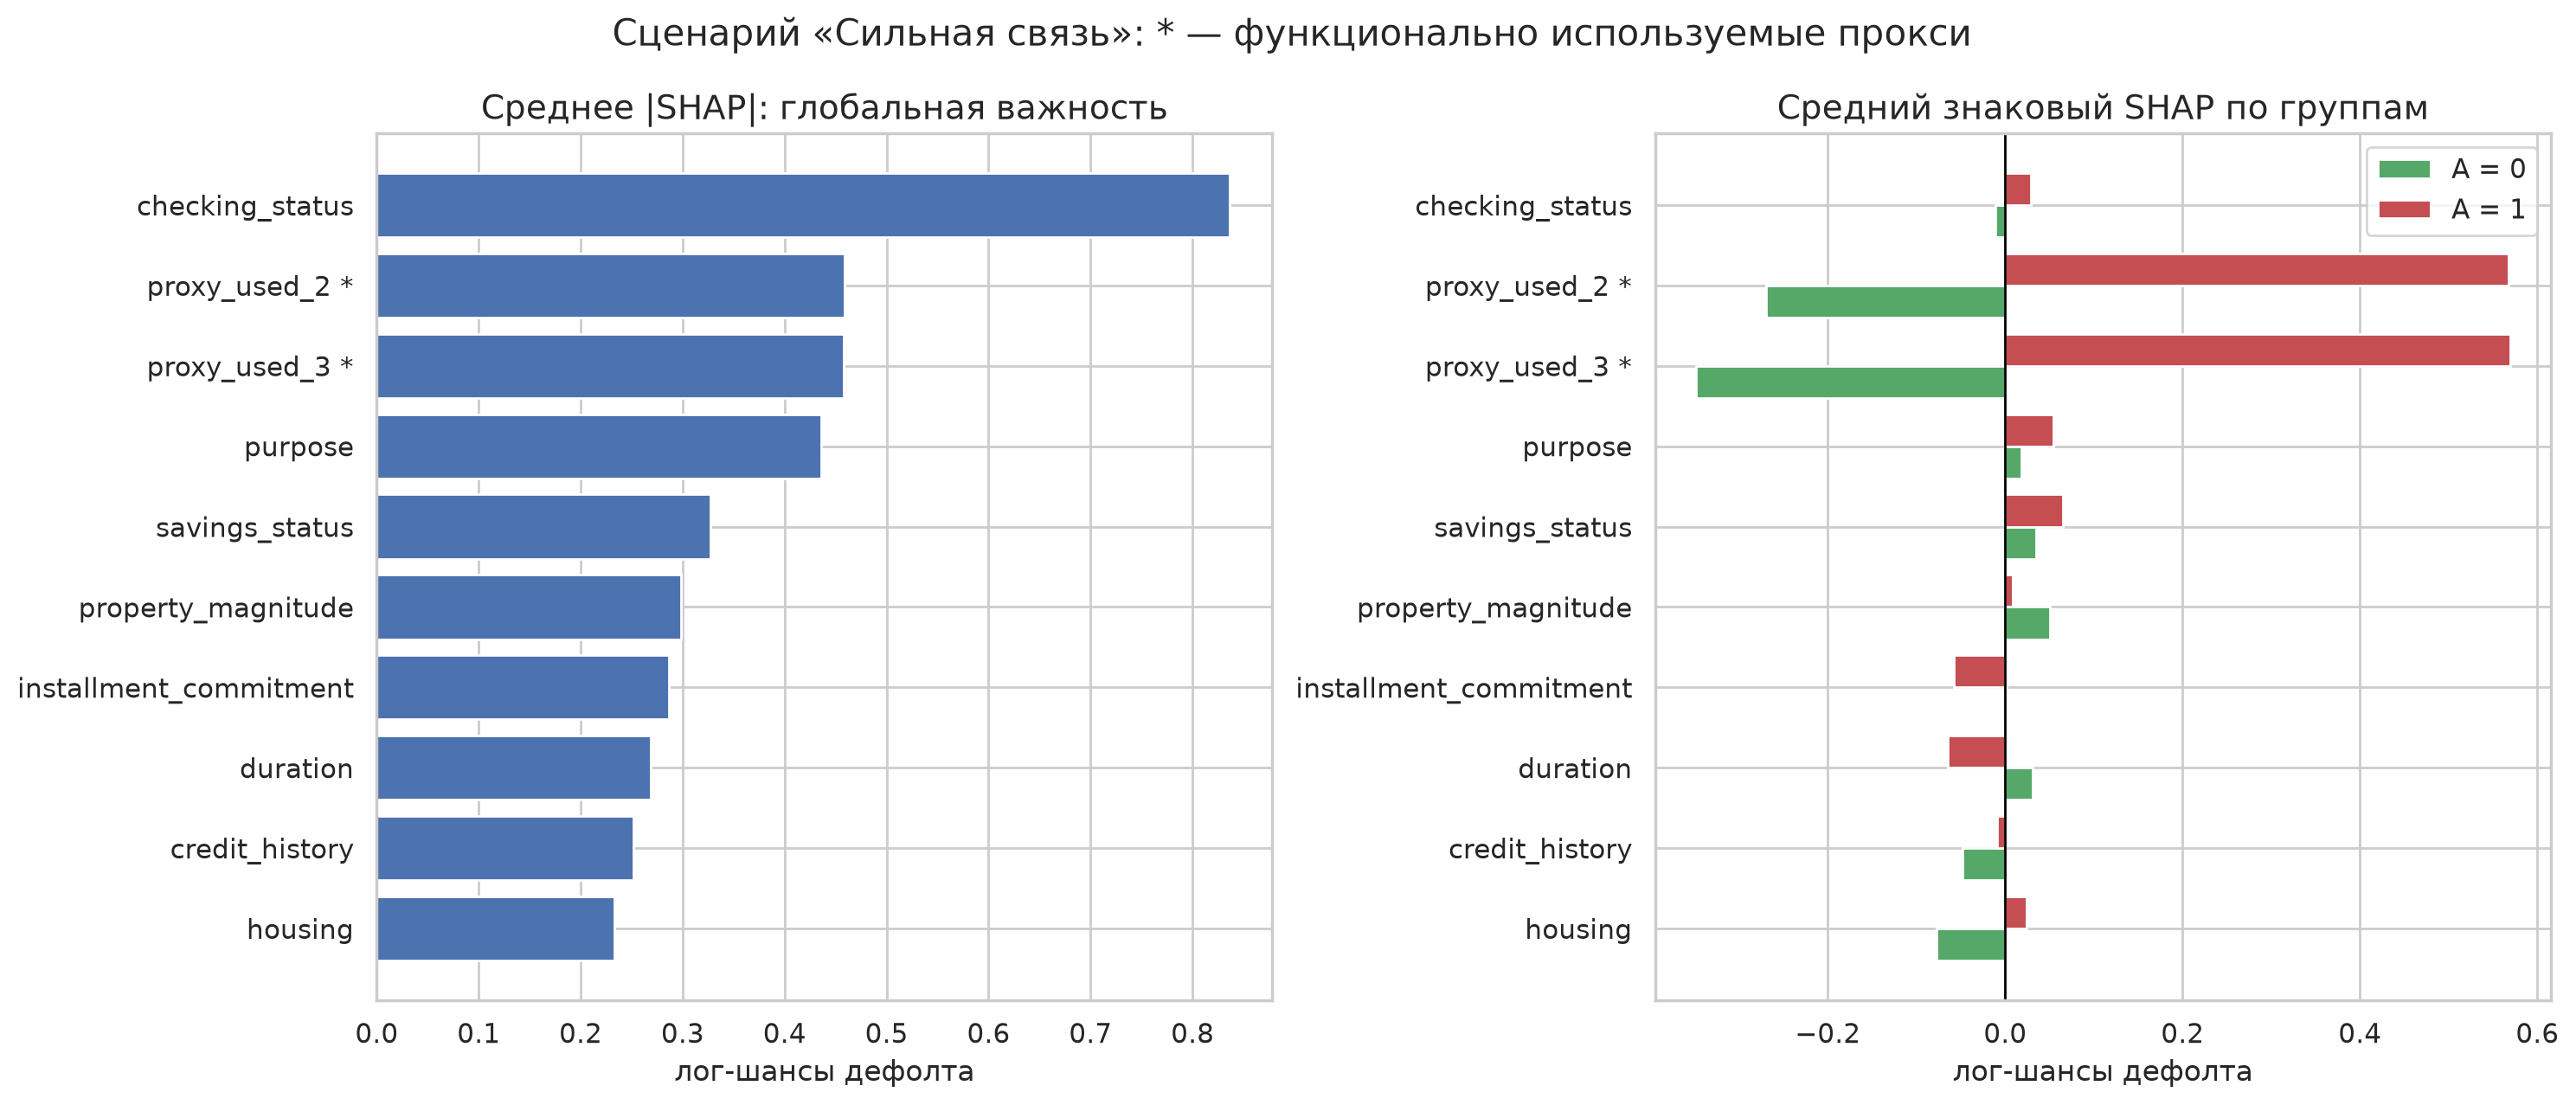
\includegraphics[width=0.95\textwidth]{fig2_signed_shap_groups.png}
\caption{Сценарий «Сильная связь» (\texttt{seed} 2026): слева — глобальная важность $\mathrm{mean}(|\mathrm{SHAP}|)$, справа — средний знаковый SHAP по группам ($*$ — признаки из $P^*$). Положительное значение соответствует росту лог-шансов дефолта.}
\label{fig:signed}
\end{figure*}

\subsection{Ограничения методики и дискуссионные вопросы}

Альтернативой пост-хок аудиту «чёрных ящиков» выступает отказ от непрозрачных моделей в пользу изначально интерпретируемых алгоритмов (логистической регрессии, скоринговых карт), на чём настаивает~\cite{rudin2019} для задач с высокой ценой ошибки. Однако переход к линейным моделям в промышленном скоринге сопряжён со снижением прогностического качества, а сама проблема признаков-прокси сохраняется и в линейных моделях, и в градиентном бустинге с монотонными ограничениями.

Проведённый эксперимент имеет следующие границы применимости: набор UCI German Credit содержит 1000 записей 1994 года и не включает отклонённые заявки (что не позволяет оценить влияние reject inference), целевые метки синтезированы для контроля эталона $P^*$, а статистические оценки получены по 5 прогонам на сценарий. Тем самым эксперимент валидирует корректность самой трёхуровневой процедуры аудита в контролируемых условиях, а не характеристики конкретного банковского портфеля.

\begin{thebibliography}{99}
\raggedright

\bibitem{barocas2016}
Barocas S., Selbst A. D. Big data's disparate impact // California Law Review. 2016. Vol. 104, № 3. P. 671--732. DOI: \url{10.15779/Z38BG31}.

\bibitem{kozodoi2022}
Kozodoi N., Jacob J., Lessmann S. Fairness in credit scoring: Assessment, implementation and profit implications // European Journal of Operational Research. 2022. Vol. 297, № 3. P. 1083--1094. DOI: \url{10.1016/j.ejor.2021.06.023}.

\bibitem{chen2024}
Chen Y., Giudici P., Liu K., Raffinetti E. Measuring fairness in credit ratings // Expert Systems with Applications. 2024. Vol. 258. Art. 125184. DOI: \url{10.1016/j.eswa.2024.125184}.

\bibitem{mishurov2023}
Мишуров С. С., Мальцева Е. В. Экономико-математическое моделирование и интеллектуальный анализ данных в задачах оценки финансовых и операционных рисков // Экономика и предпринимательство. 2023. № 5 (154). С. 1142--1147. EDN: XZXCVB.

\bibitem{lundberg2017}
Lundberg S. M., Lee S.-I. A Unified Approach to Interpreting Model Predictions // Advances in Neural Information Processing Systems (NeurIPS). 2017. Vol. 30. P. 4765--4774.

\bibitem{lundberg2020}
Lundberg S. M. et al. From local explanations to global understanding with explainable AI for trees // Nature Machine Intelligence. 2020. Vol. 2, № 1. P. 56--67.

\bibitem{ribeiro2016}
Ribeiro M. T., Singh S., Guestrin C. «Why Should I Trust You?»: Explaining the Predictions of Any Classifier // Proceedings of the 22nd ACM SIGKDD International Conference on Knowledge Discovery and Data Mining. 2016. P. 1135--1144. DOI: \url{10.1145/2939672.2939778}.

\bibitem{demin2026}
Демин Н. И., Матвеев В. С. Применение методов объяснимого искусственного интеллекта и анализа вклада признаков в прикладных задачах классификации // Искусственный интеллект в промышленных, коммерческих, медицинских и финансовых приложениях: сборник статей научно-технического семинара кафедры инженерной кибернетики / под ред. Р. Н. Садекова. М.: НИТУ «МИСИС», 2026. URL: \url{https://sadekov.su/}.

\bibitem{abramov2026}
Абрамов И. В. Сравнительный анализ методов интерпретации сложных ML-моделей в задачах оценивания рисков // Искусственный интеллект в промышленных, коммерческих, медицинских и финансовых приложениях: сборник статей научно-технического семинара кафедры инженерной кибернетики / под ред. Р. Н. Садекова. М.: НИТУ «МИСИС», 2026. URL: \url{https://sadekov.su/}.

\bibitem{slack2020}
Slack D., Hilgard S., Jia E., Singh S., Lakkaraju H. Fooling LIME and SHAP: Adversarial Attacks on Post hoc Explanation Methods // Proceedings of the AAAI/ACM Conference on AI, Ethics, and Society (AIES). 2020. P. 180--186. DOI: \url{10.1145/3375627.3375830}.

\bibitem{hardt2016}
Hardt M., Price E., Srebro N. Equality of Opportunity in Supervised Learning // Advances in Neural Information Processing Systems (NeurIPS). 2016. Vol. 29. P. 3315--3323.

\bibitem{verma2018}
Verma S., Rubin J. Fairness Definitions Explained // Proceedings of the International Workshop on Software Fairness (FairWare). 2018. P. 1--7. DOI: \url{10.1145/3194770.3194776}.

\bibitem{kumar2020}
Kumar I. E., Venkatasubramanian S., Scheidegger C., Friedler S. Problems with Shapley-value-based explanations as feature importance measures // Proceedings of the 37th International Conference on Machine Learning (ICML). 2020. Vol. 119. P. 5491--5500.

\bibitem{wachter2018}
Wachter S., Mittelstadt B., Russell C. Counterfactual Explanations without Opening the Black Box: Automated Decisions and the GDPR // Harvard Journal of Law \& Technology. 2018. Vol. 31, № 2. P. 841--887.

\bibitem{germancredit}
Hofmann H. Statlog (German Credit Data) // UCI Machine Learning Repository. 1994. DOI: \url{10.24432/C5NC77}.

\bibitem{rudin2019}
Rudin C. Stop explaining black box machine learning models for high stakes decisions and use interpretable models instead // Nature Machine Intelligence. 2019. Vol. 1, № 5. P. 206--215.

\end{thebibliography}

\end{document}